%
% ---------- header -----------------------------------------------------------
%
% project       kaneton
%
% license       kaneton
%
% file          /home/mycure/kane...ernels/virtualization/virtualization.tex
%
% created       julien quintard   [wed may 16 19:28:59 2007]
% updated       julien quintard   [tue may  5 10:49:43 2009]
%

%
% ---------- setup ------------------------------------------------------------
%


%
% title
%

\title{Virtualisation}

%
% table of contents at the beginning of each section
%

\AtBeginSection[]
{
  \begin{frame}<beamer>
    \frametitle{Outline}

    \begin{multicols}{2}
      \tableofcontents[current,hidesubsections]
    \end{multicols}
  \end{frame}
}

%
% table of contents at the beginning of each subsection
%

\AtBeginSubsection[]
{
  \begin{frame}<beamer>
    \frametitle{Outline}

    \begin{multicols}{2}
      \tableofcontents[current,hidesubsections]
    \end{multicols}
  \end{frame}
}

%
% document
%

\begin{document}

%
% title frame
%

\begin{frame}
  \titlepage
\end{frame}

%
% outline frame
%

\begin{frame}
  \frametitle{Outline}

  \begin{multicols}{2}
    \tableofcontents
  \end{multicols}
\end{frame}

  % -)


\section{Introduction}
\begin{frame}
\frametitle{Introduction}
\begin{itemize}
\item The Virtualisation platform create a abstraction in order to run multiple OS or system on the same physical machine.
\item Virtualisation exists since a long time, 1960s with IBM.
\item There is multiple level of virtualisation.
\item Nowadays the success of the virtualisation software made the hardware vendor to do some research to add hardware assistance.
\end{itemize}
\end{frame}

\section{Terminology}
\subsection{Binary translation}
\begin{frame}
\frametitle{Binary translation}
\begin{itemize}
\item This is basically a virtual machine.
\item All the code is disassembled and translated.
\item It's really slow but works without any hardware support.
\item Example: QEMU
\end{itemize}
\end{frame}

\subsection{Binary patching}
\begin{frame}
\frametitle{Binary Translation}
\begin{itemize}
  \item Load the binaries into memory and modify the code directly.
  \item Replace the special instructions with specific calls, (for instance ldtr).
  \item It's quite slow and force to parse all the code before executing
  it.
  \item Like the binary translation this techniques doesn�t require any hardware support.
  \item Example: VMWare workstation
\end{itemize}
\end{frame}

\subsection{Emulation}
\begin{frame}
\frametitle{Emulation}
\begin{itemize}
\item The two previous techniques can be consider as emulation.
\item We usually talk about emulation for hardware emulation, not for the code being executed.
\item In a virtualised environment most of the hardware is emulated because it's an abstraction.
\item Example: QEMU is a hardware emulation software
\end{itemize}
\end{frame}

\subsection{Virtualisation}
\begin{frame}
\frametitle{Virtualisation}
\begin{itemize}
\item We often talk about virtualisation when there is hardware assistance, or the techniques in place don't have that much overhead.
\item It's usually a mix of all the previous techniques.
\item Example: Xen, VMWare ESX
\end{itemize}
\end{frame}

\section{Different kind of virtualisation}
\subsection{Paravirtualisation}
\begin{frame}
\frametitle{Paravirtualisation}
\begin{itemize}
\item The kernel is modified in order to run inside a virtualised environment.
\item So far it's mainly for Linux running under Xen.
\item You replace all hardware calls with syscalls (hypercall in this case), like (ldtr, gtdr, cr3, \ldots ).
\item The overhead compared with native is less then 5\%.
\item Linux have a paravirtualisation interface since 2.6.22 (called pvops).
\item Xen paravirtualized guest work since 2.6.24.
\item This technique doesn�t required any special hardware.
\end{itemize}
\end{frame}

\begin{frame}[fragile]
\frametitle{CPU pvops (arch/x86/include/asm/paravirt.h)}
\begin{verbatim}
struct pv_cpu_ops {
        /* hooks for various privileged instructions */
[...]
        unsigned long (*read_cr0)(void);
        void (*write_cr0)(unsigned long);
        unsigned long (*read_cr4_safe)(void);
        unsigned long (*read_cr4)(void);
        void (*write_cr4)(unsigned long);
#ifdef CONFIG_X86_64
        unsigned long (*read_cr8)(void);
        void (*write_cr8)(unsigned long);
#endif
        /* Segment descriptor handling */
        void (*load_tr_desc)(void);
        void (*load_gdt)(const struct desc_ptr *);
        void (*load_idt)(const struct desc_ptr *);
        void (*store_gdt)(struct desc_ptr *);
        void (*store_idt)(struct desc_ptr *);
        void (*set_ldt)(const void *desc, unsigned entries);
[...]
        /* cpuid emulation, mostly so that caps bits can be disabled */
        void (*cpuid)(unsigned int *eax, unsigned int *ebx,
                      unsigned int *ecx, unsigned int *edx);
[...]
}
\end{verbatim}
\end{frame}
\begin{frame}[fragile]
\frametitle{MMU pvops (arch/x86/include/asm/paravirt.h)}
\begin{verbatim}
struct pv_mmu_ops {
        unsigned long (*read_cr3)(void);
        void (*write_cr3)(unsigned long);
        void (*activate_mm)(struct mm_struct *prev,
                            struct mm_struct *next);
        void (*dup_mmap)(struct mm_struct *oldmm,
                         struct mm_struct *mm);
        void (*exit_mmap)(struct mm_struct *mm);
        /* TLB operations */
        void (*flush_tlb_user)(void);
        void (*flush_tlb_kernel)(void);
        /* Hooks for allocating and freeing a pagetable top-level */
        int  (*pgd_alloc)(struct mm_struct *mm);
        void (*pgd_free)(struct mm_struct *mm, pgd_t *pgd);
        /* Pagetable manipulation functions */
        void (*set_pte)(pte_t *ptep, pte_t pteval);
        void (*set_pte_at)(struct mm_struct *mm, unsigned long addr,
                           pte_t *ptep, pte_t pteval);
        void (*set_pmd)(pmd_t *pmdp, pmd_t pmdval);
        void (*pte_update)(struct mm_struct *mm, unsigned long addr,
                           pte_t *ptep);
[...]
}
\end{verbatim}
\end{frame}

\subsection{Hardware assisted virtualisation (HVM)}
\begin{frame}
\frametitle{Hardware assisted virtualisation (HVM)}
\begin{itemize}
\item A new set of instruction and table in order to do virtualisation in a more efficient way.
\item Most of virtualisation solution required those processor feature like KVM.
\item Xen needs that in order to run unmodified kernel like windows.
\end{itemize}
\end{frame}

\section{Technology (hardware virtualisation)}
\subsection{VMX}
\begin{frame}
\frametitle{Intel VMX}
\begin{itemize}
\item Codename "Vanderpool Technology"
\item Also called VT-x
\item Start with Pentium 4 662
\item It's a processor feature.
\item VMENTER, VMEXIT, VMCS, VMM.
\end{itemize}
\end{frame}
\subsection{SVM}
\begin{frame}
\frametitle{AMD SVM}
\begin{itemize}
\item Also called Pacifica or AMD-V
\item Release the 23rd May 2006
\item Real mode support.
\end{itemize}
\end{frame}

\section{Design}
\subsection{Type 1}
\begin{frame}
\frametitle{Type 1}
\begin{itemize}
\item The VMM runs under every thing, it's the first to boot on the
system.
\item We called that bar-metal hypervisor.
\item As close to the hardware as possible.
\item On the top of it there are, privileged and non privileged virtual
machine.
\item It's more secure.
\item In this case the hypervisor usually takes care of:
\begin{itemize}
\item Memory management
\item Interrupts
\item Virtual machine scheduling
\end{itemize}
\item Software: Xen, VMWare ESX.
\end{itemize}
\end{frame}

\begin{frame}
\begin{center}
\frametitle{Type 1 hypervisor}
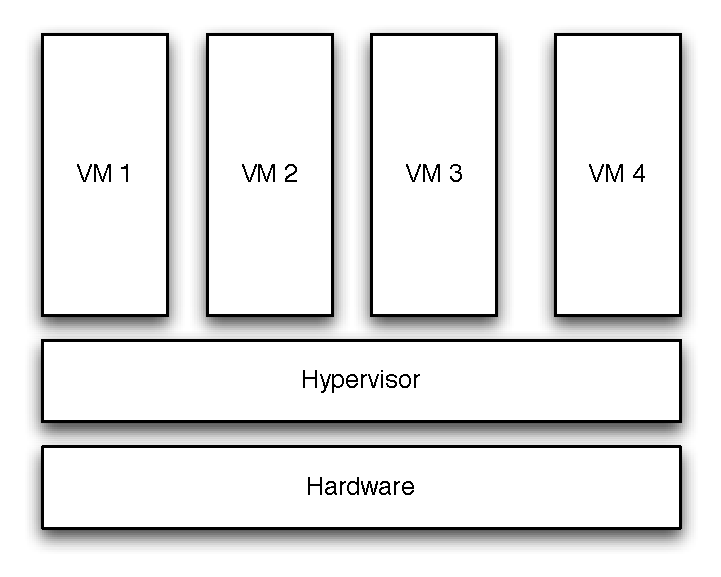
\includegraphics[height=150pt]{\figurepath/figures/type_1}
\end{center}
\end{frame}


\subsection{Type 2}
\begin{frame}
\frametitle{Type 2}
\begin{itemize}
\item The VMM run on the top of a existing operating system.
\item This is generally a kernel module.
\item The VMM can be compromised through the OS.
\item Much easier to install.
\item Software: KVM, VMWare Fusion, Paralleles, virtual box, \ldots
\end{itemize}
\end{frame}

\begin{frame}
\frametitle{Type 2 hypervisor}
\begin{center}
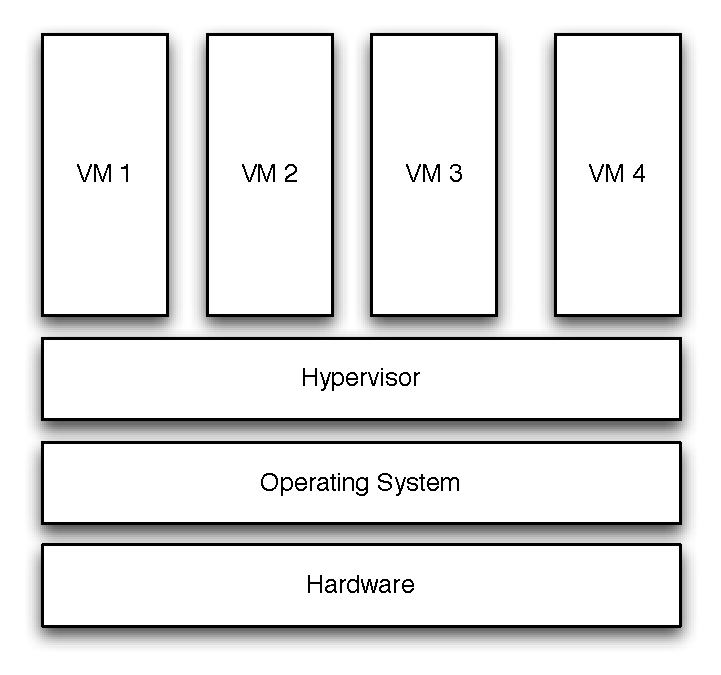
\includegraphics[height=150pt]{\figurepath/figures/type_2}
\end{center}
\end{frame}

\section{Device management}
\subsection{Emulation}
\begin{frame}
\frametitle{Device emualtion}
\begin{itemize}
\item When a virtual machine runs we need to emulate all the hardware.
\item KVM and Xen use qemu for that.
\item VMWare and virtual box got there own device emulator.
\item This layer is reponsible for all the hardware abstraction.
\item This is usally very slow and the bottleneck of the hole system.
\end{itemize}
\end{frame}

\subsection{PV driver}
\begin{frame}
\frametitle{PV driver}
\begin{itemize}
\item It's called VMWare tools, xenTools or virtual box Tools.
\item Instead of using the emulated device path, the tools load some driver that talks directly with the virtualisation layer.
\item That technique completely by-pass the emulation layer.
\item It's very useful for high speed device, like hard drive or network
card.
\item You have to write a driver of each kind of OS you want to virtualise so it's not generic.
\end{itemize}
\end{frame}

\section{Memory management}
\subsection{Shadow page table}
\begin{frame}
\frametitle{Shadow page table}
\begin{overlayarea}{10cm}{10cm}
\only<1> {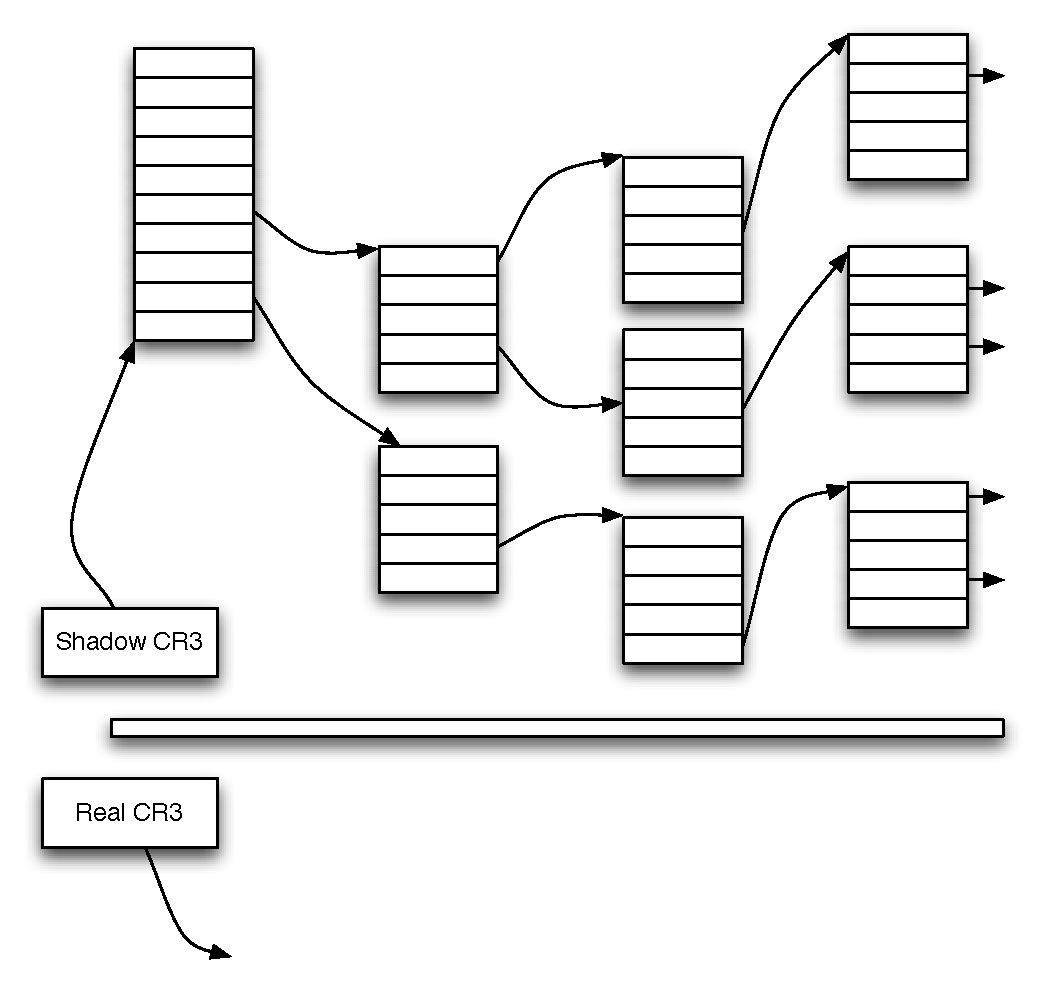
\includegraphics[height=6cm]{\figurepath/figures/shadow_page_table_1}}
\only<2> {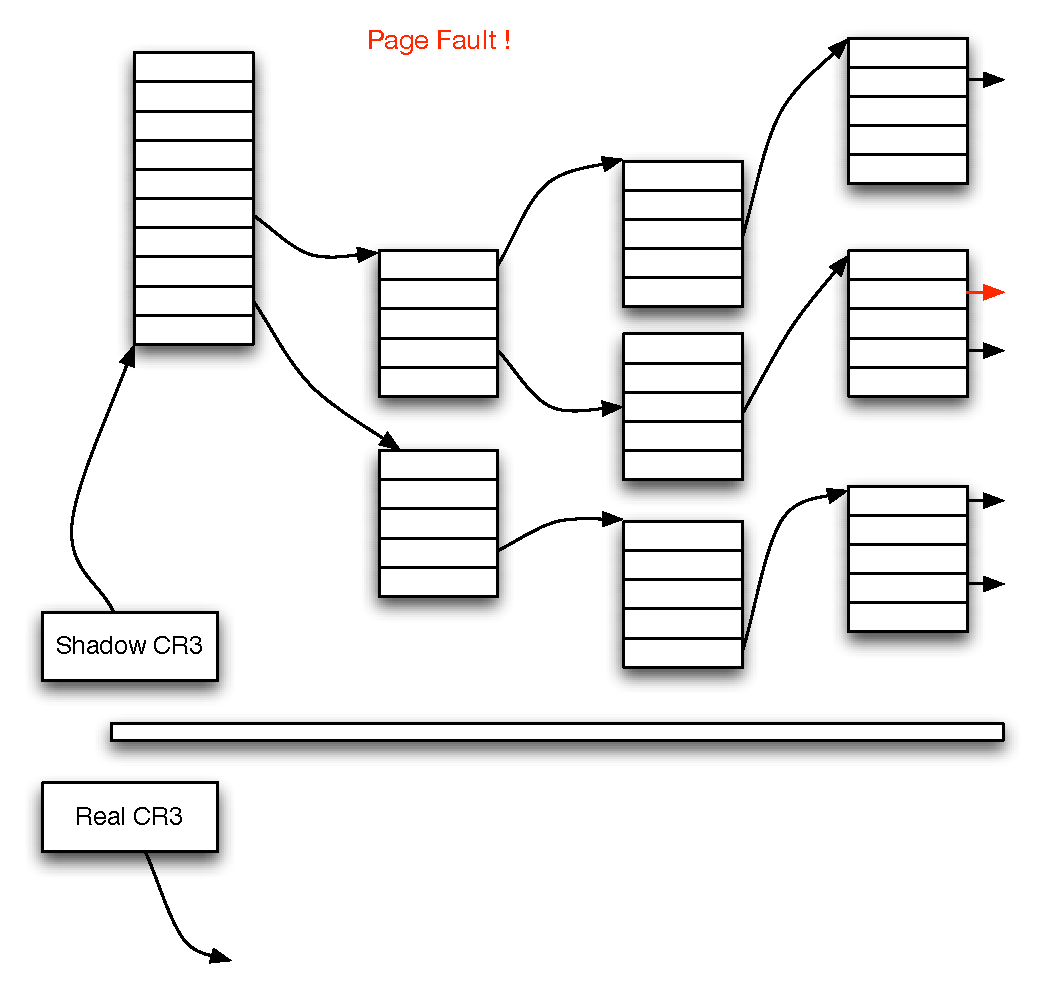
\includegraphics[height=6cm]{\figurepath/figures/shadow_page_table_2}}
\only<3> {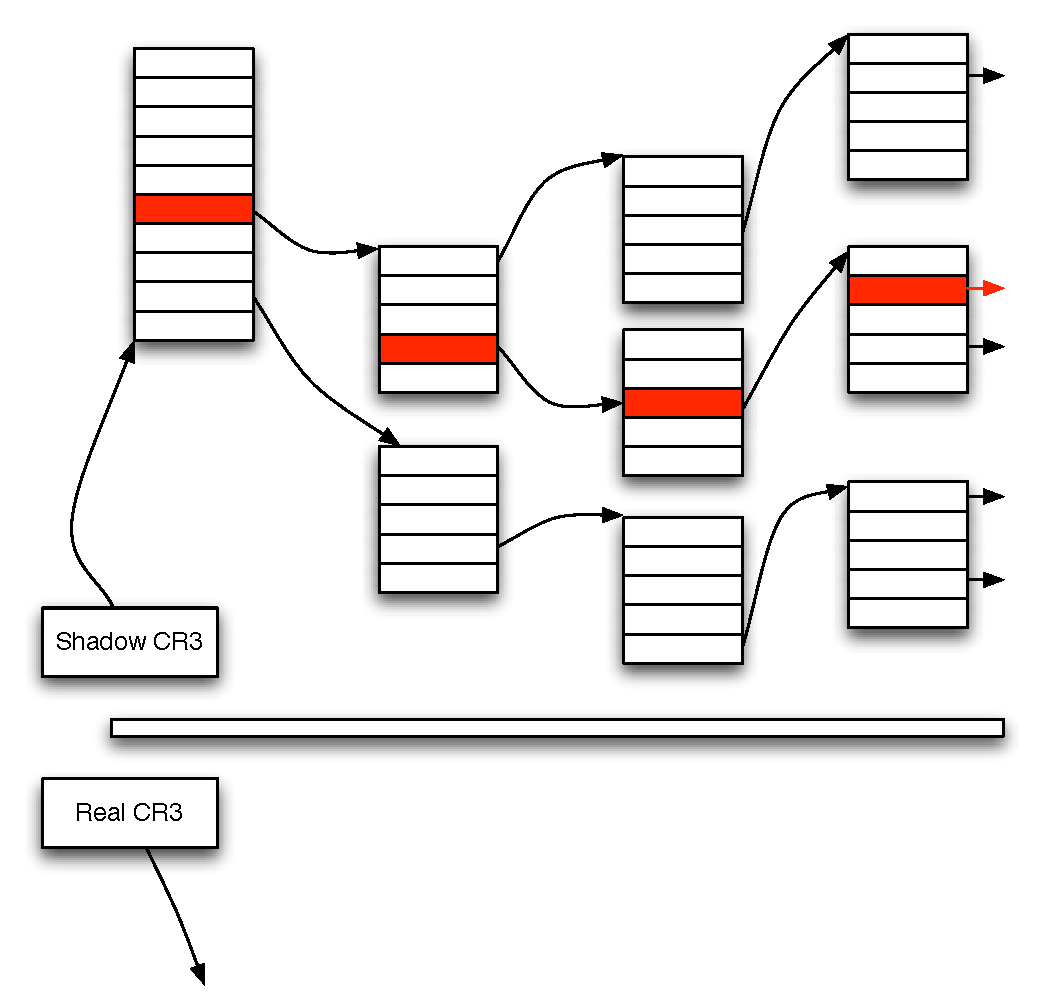
\includegraphics[height=6cm]{\figurepath/figures/shadow_page_table_3}}
\only<4> {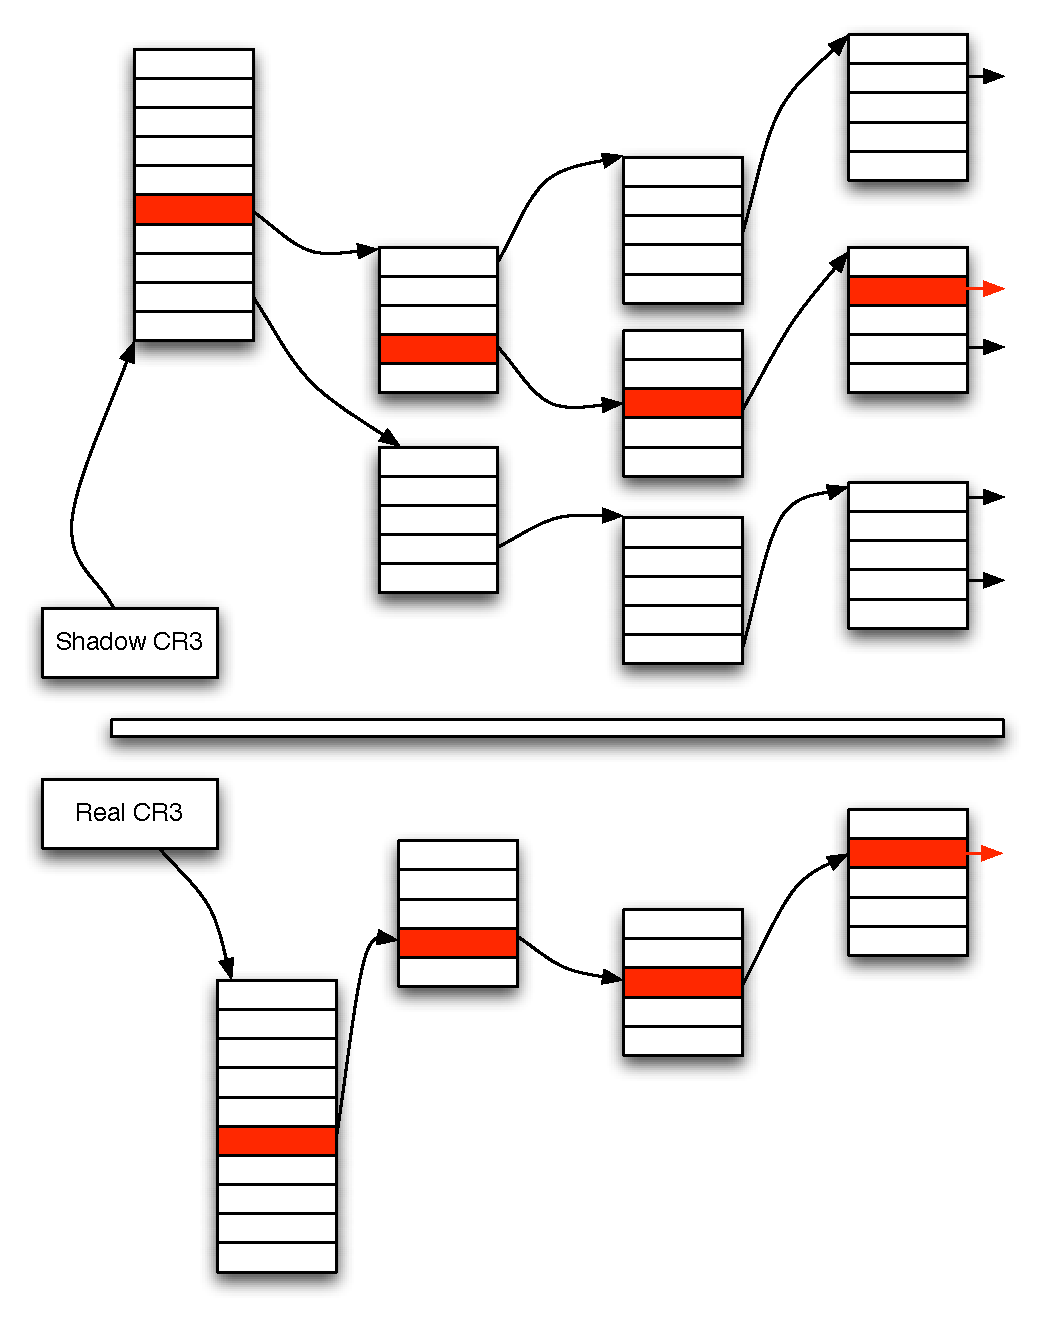
\includegraphics[height=6cm]{\figurepath/figures/shadow_page_table_4}}
\only<5> {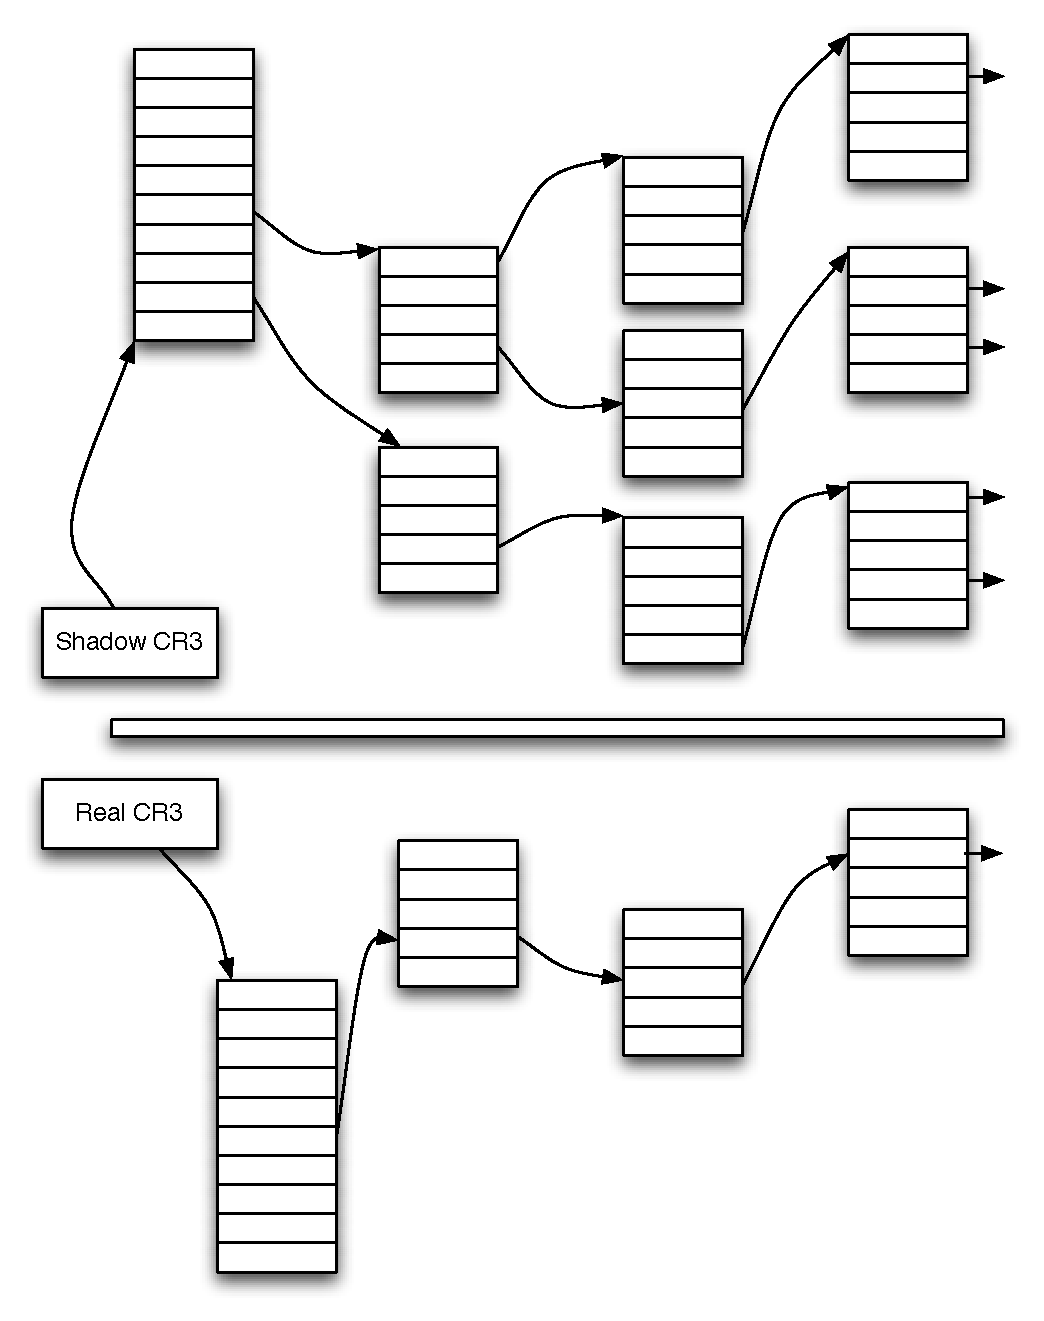
\includegraphics[height=6cm]{\figurepath/figures/shadow_page_table_5}}
\only<6> {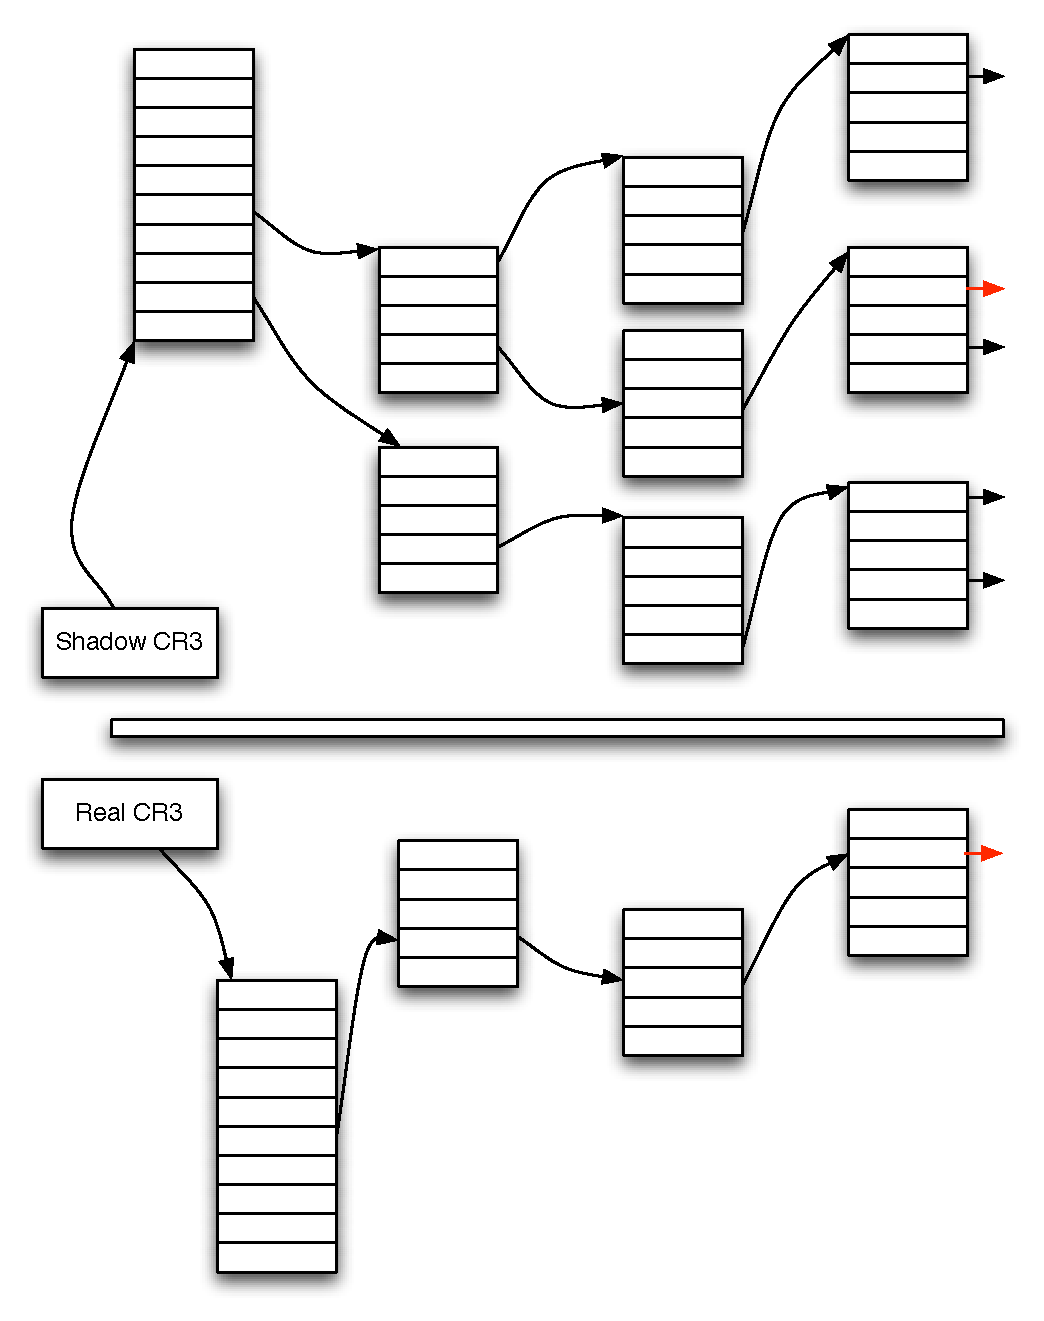
\includegraphics[height=6cm]{\figurepath/figures/shadow_page_table_6}}
\only<7> {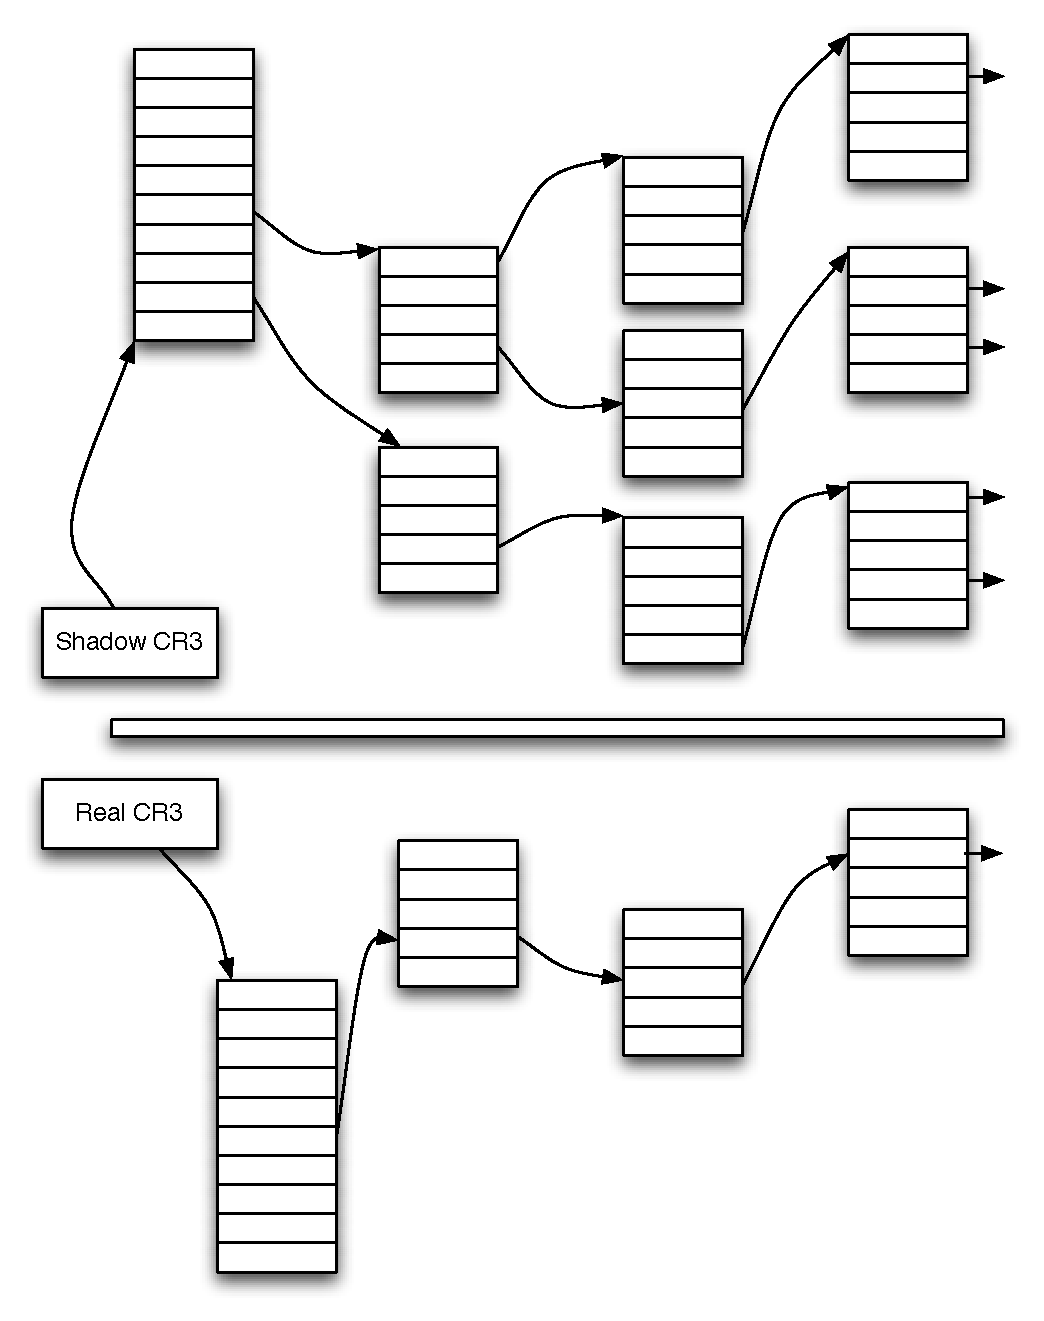
\includegraphics[height=6cm]{\figurepath/figures/shadow_page_table_7}}
\only<8> {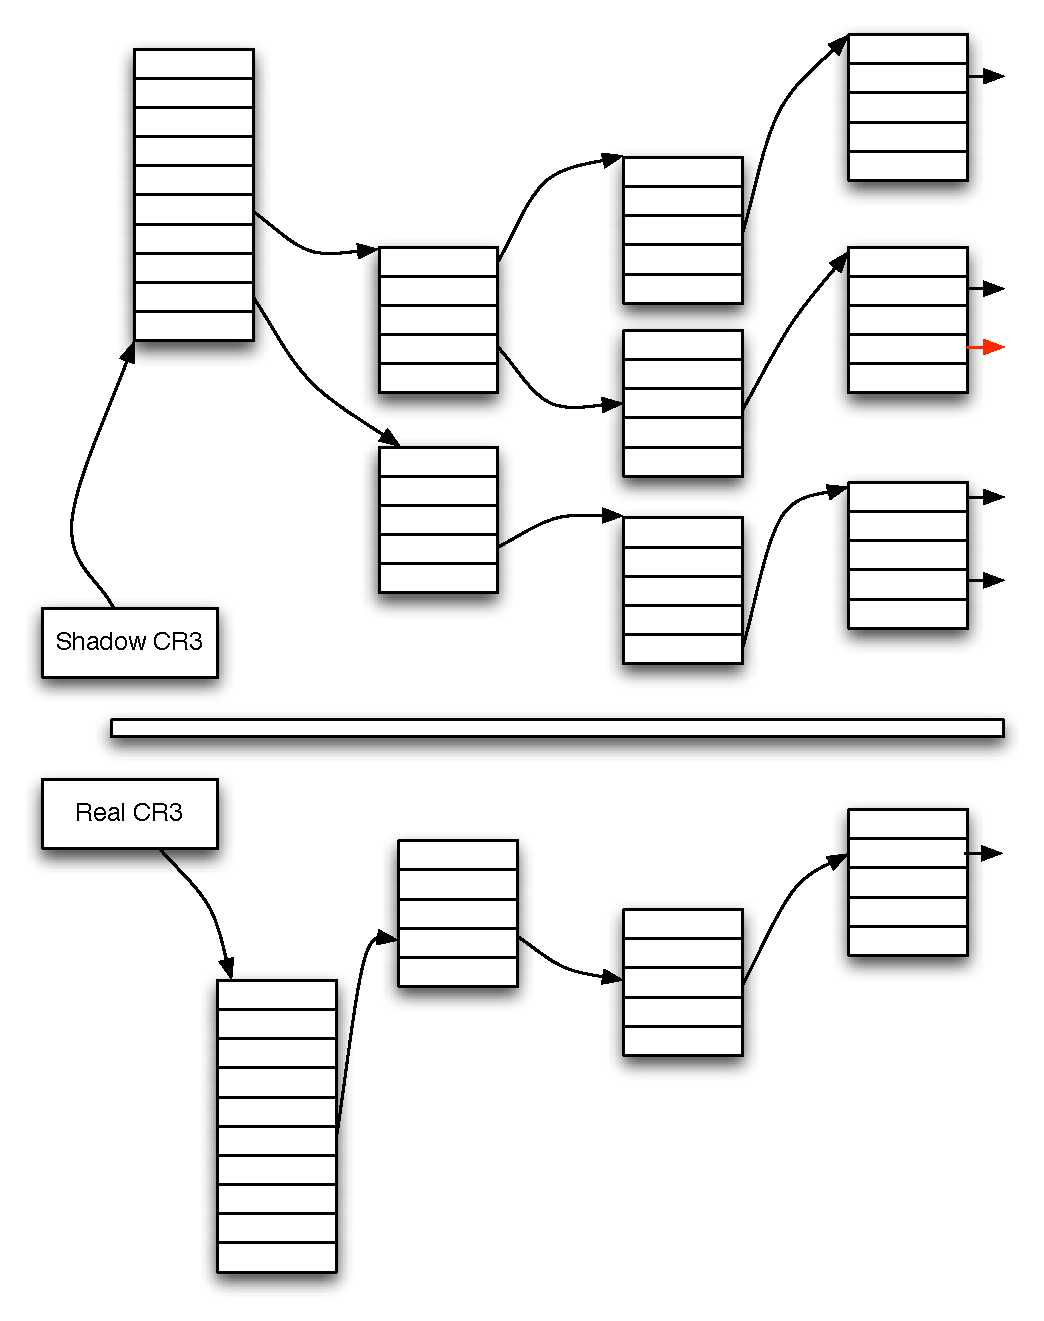
\includegraphics[height=6cm]{\figurepath/figures/shadow_page_table_8}}
\only<9> {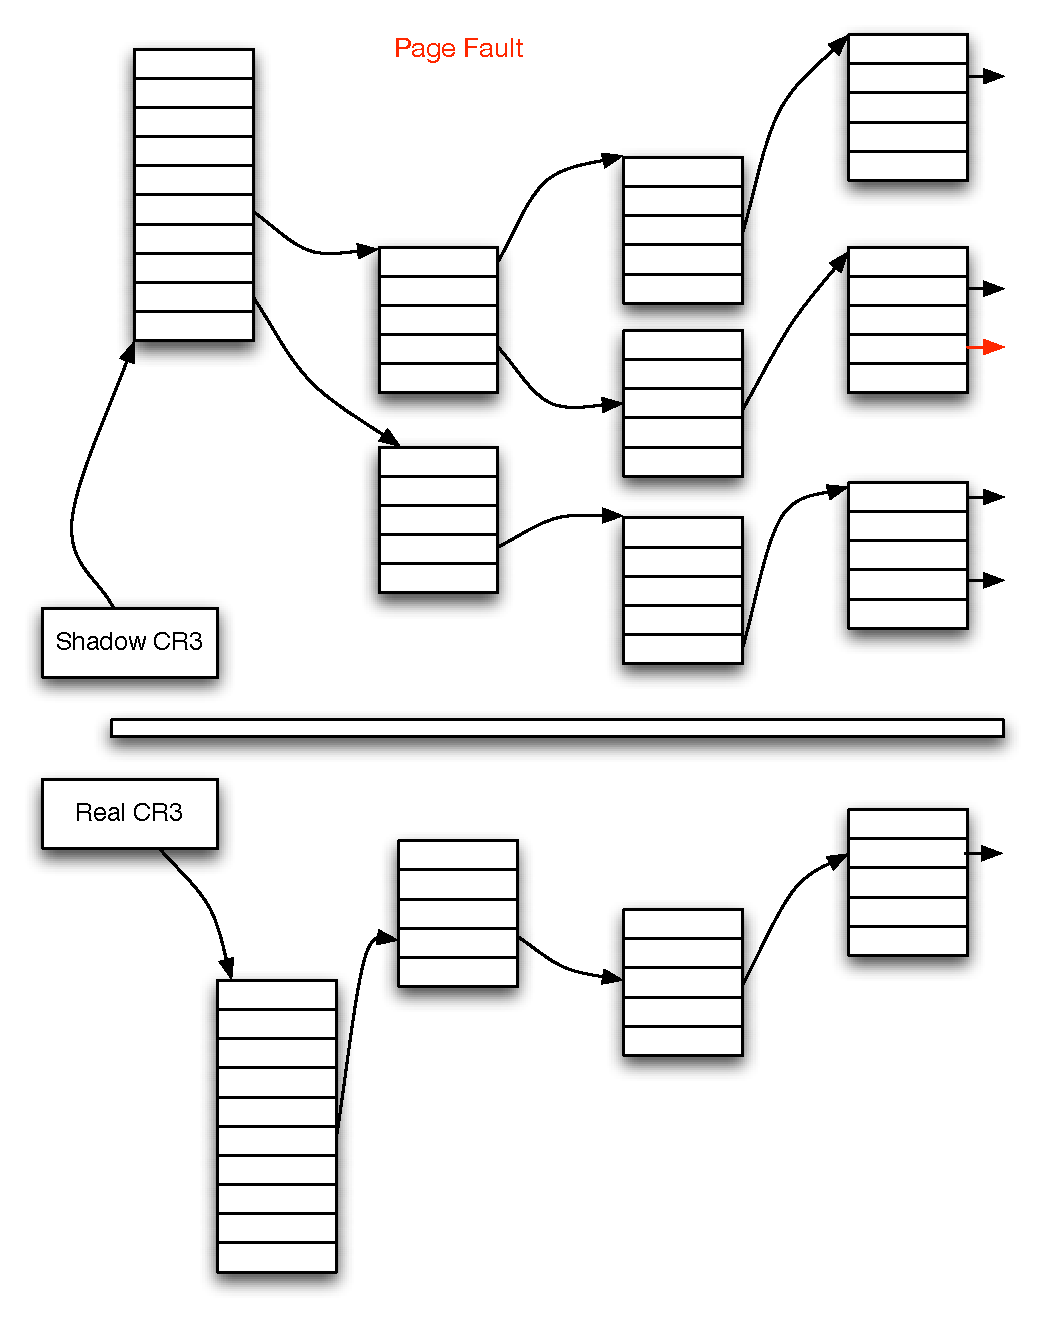
\includegraphics[height=6cm]{\figurepath/figures/shadow_page_table_9}}
\only<10>{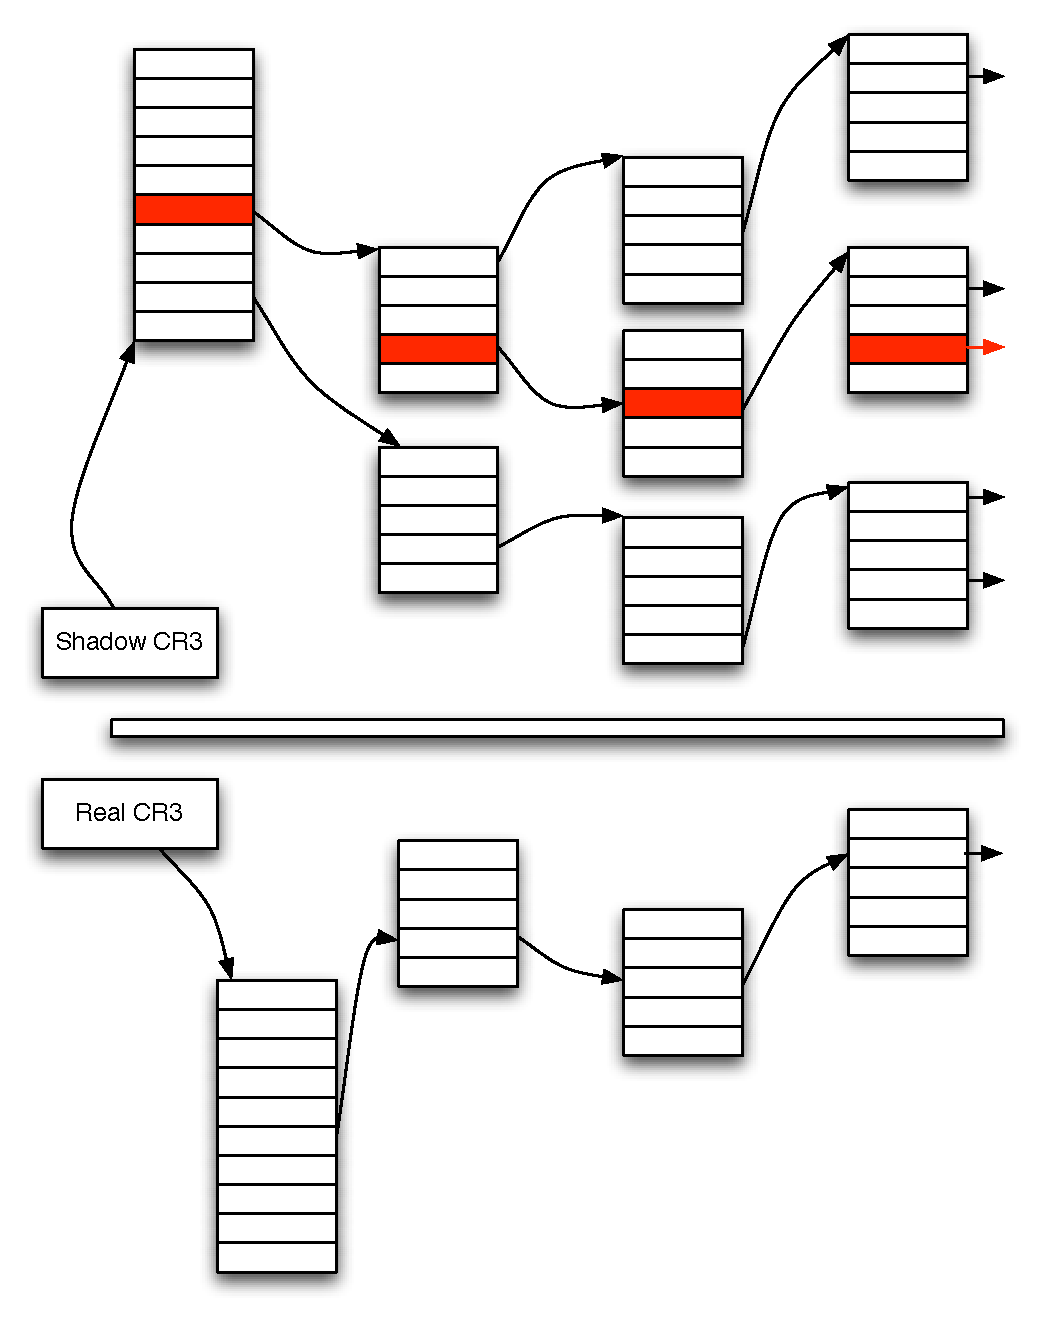
\includegraphics[height=6cm]{\figurepath/figures/shadow_page_table_10}}
\only<11>{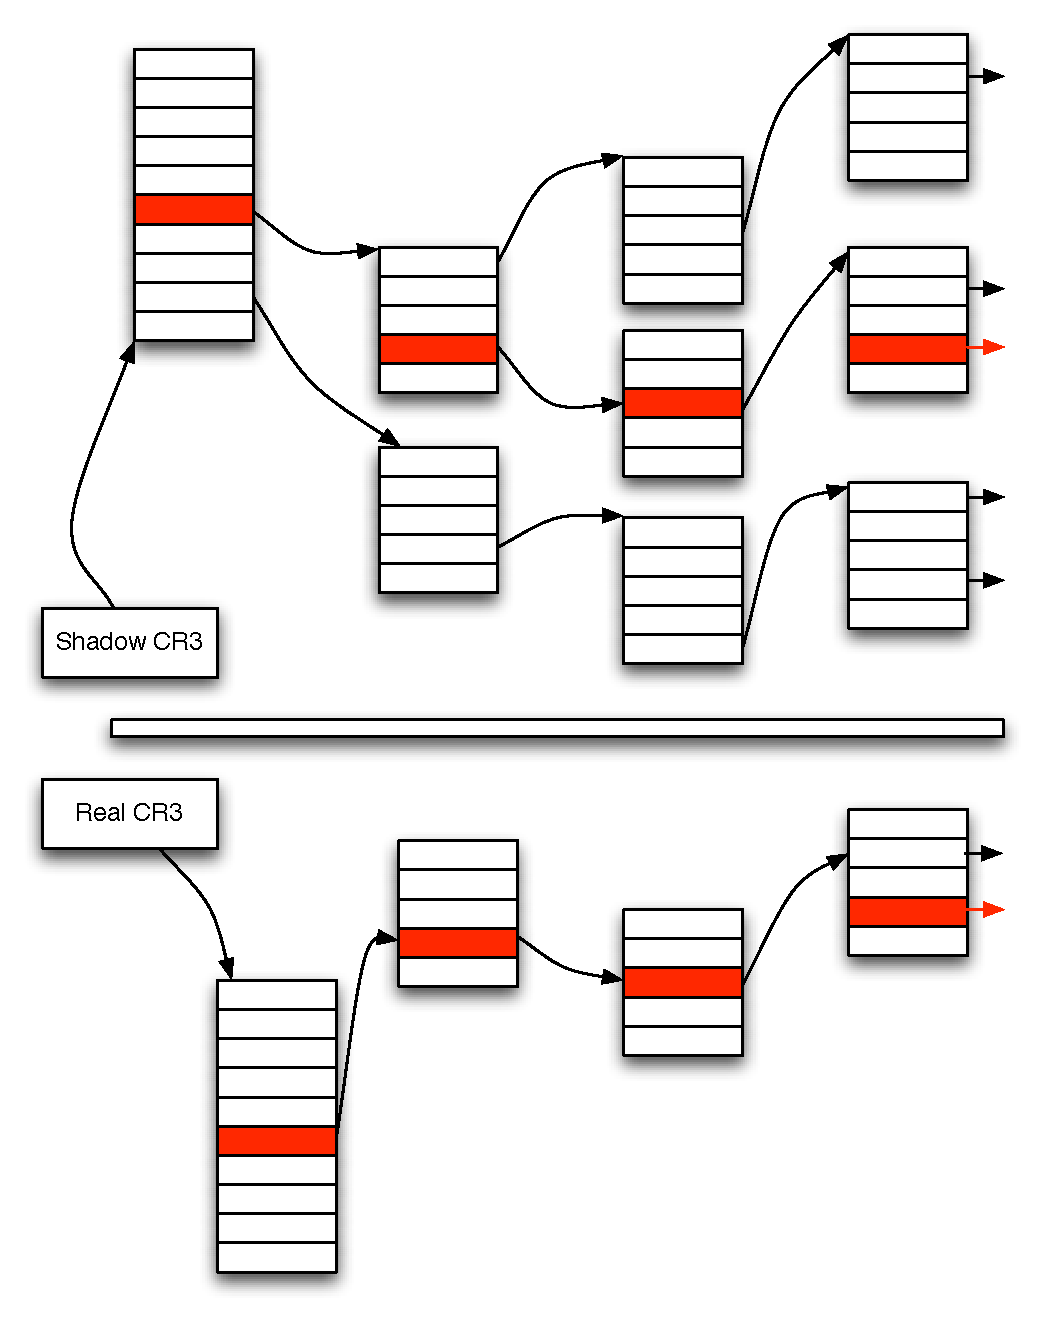
\includegraphics[height=6cm]{\figurepath/figures/shadow_page_table_11}}
\only<12>{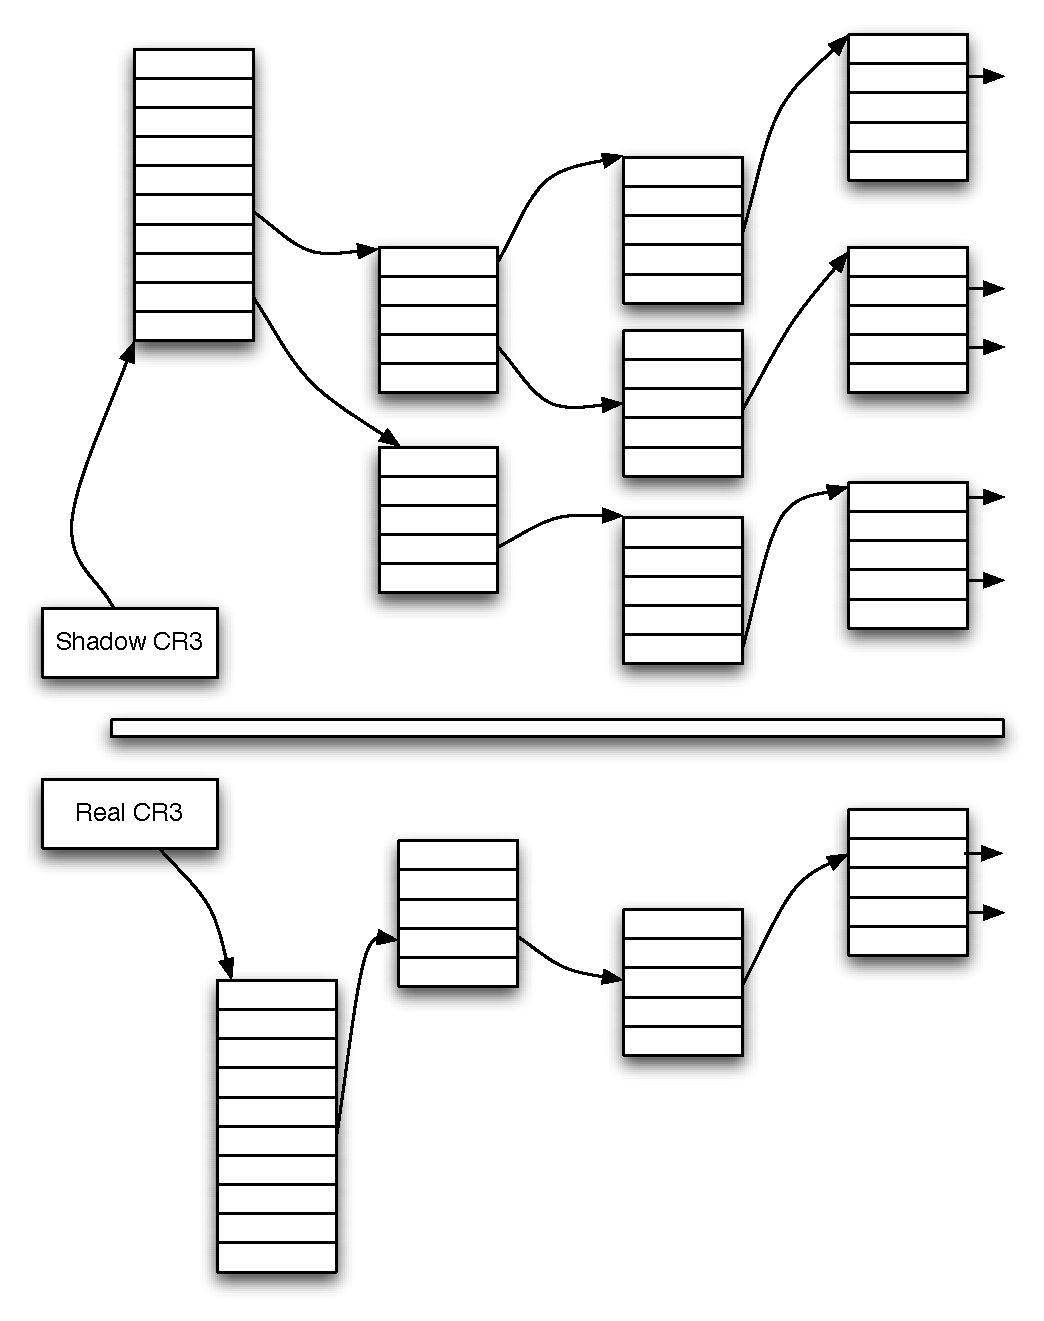
\includegraphics[height=6cm]{\figurepath/figures/shadow_page_table_12}}
\only<13>{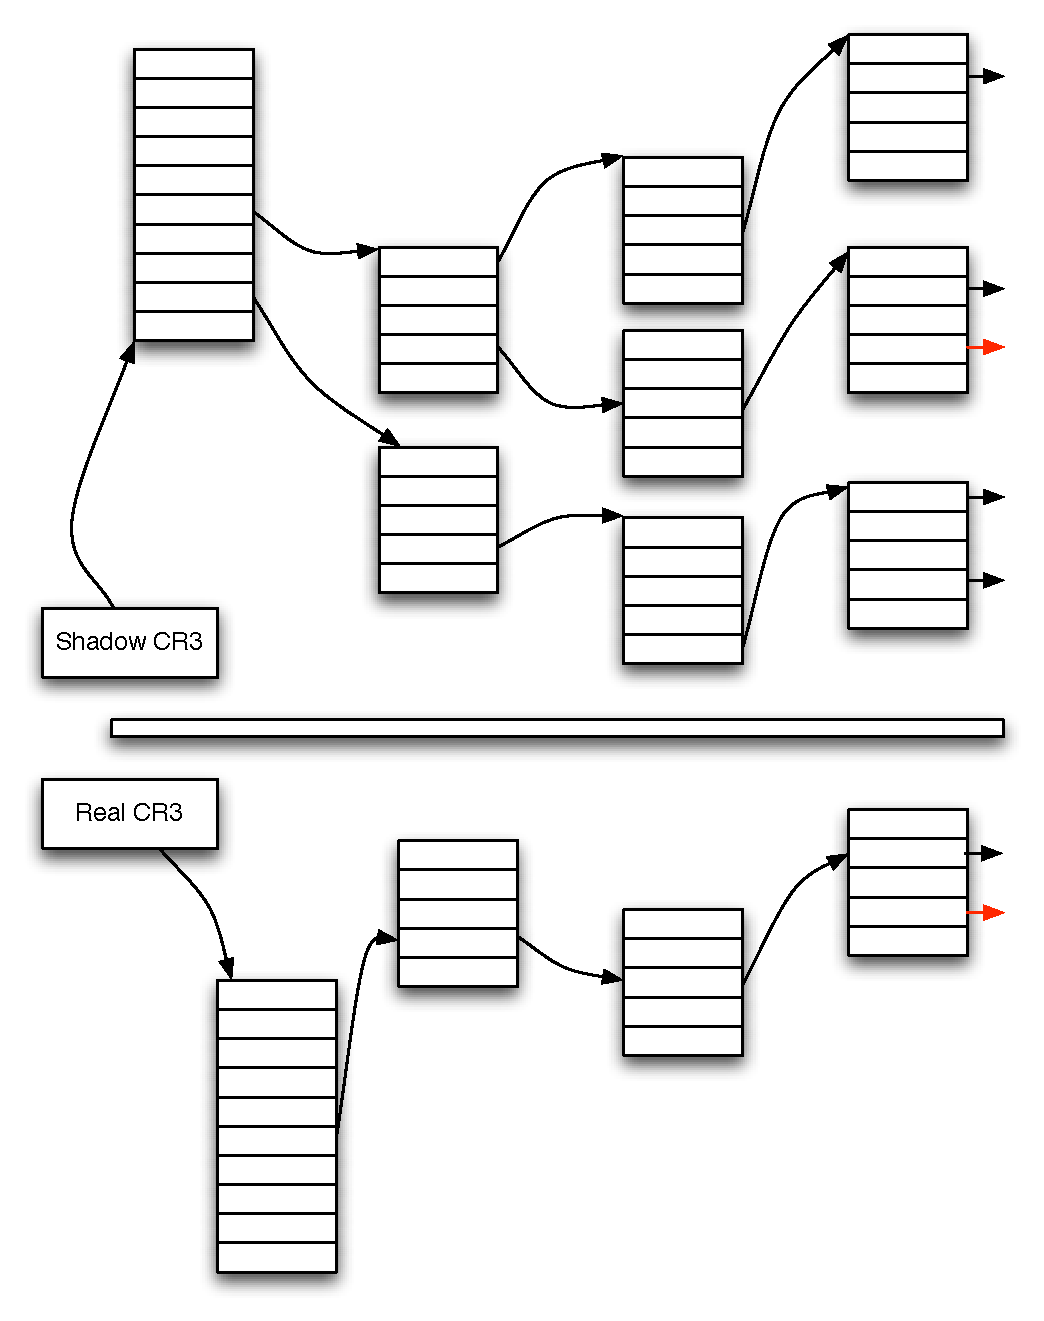
\includegraphics[height=6cm]{\figurepath/figures/shadow_page_table_13}}
\only<14>{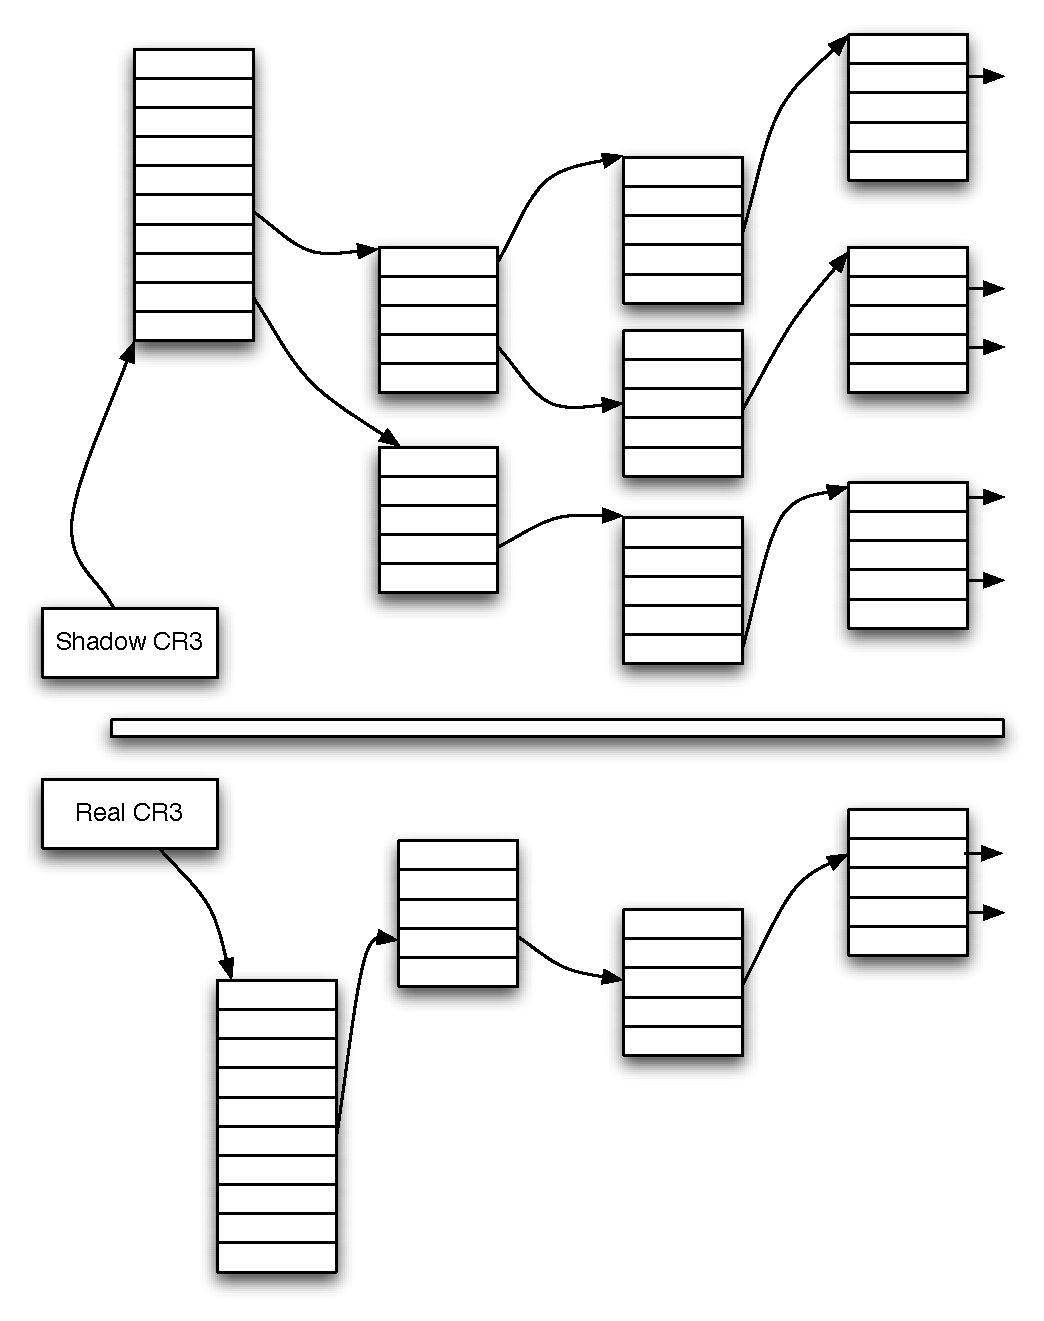
\includegraphics[height=6cm]{\figurepath/figures/shadow_page_table_14}}
\end{overlayarea}
\end{frame}

\subsection{EPT}
\begin{frame}
\frametitle{EPT}
\begin{itemize}
\item Extended page table.
\item This is hardware accelerated page table.
\item Comes with the Nehalem.
\end{itemize}
\end{frame}

\end{document}

